%%%%%%%%%%%%%%%%%%%%%%%%%%%%%%%%%%%%%%%%%%%%%%%%%%%%%%%%%%%%%%%%%%%%%%
% LaTeX Template: Beamer arrows
%
% Source: http://www.texample.net/
% Feel free to distribute this template, but please keep the
% referal to TeXample.net.
% Date: Nov 2006
% 
%%%%%%%%%%%%%%%%%%%%%%%%%%%%%%%%%%%%%%%%%%%%%%%%%%%%%%%%%%%%%%%%%%%%%%
% How to use writeLaTeX: 
%
% You edit the source code here on the left, and the preview on the
% right shows you the result within a few seconds.
%
% Bookmark this page and share the URL with your co-authors. They can
% edit at the same time!
%
% You can upload figures, bibliographies, custom classes and
% styles using the files menu.
%
% If you're new to LaTeX, the wikibook is a great place to start:
% http://en.wikibooks.org/wiki/LaTeX
%
%%%%%%%%%%%%%%%%%%%%%%%%%%%%%%%%%%%%%%%%%%%%%%%%%%%%%%%%%%%%%%%%%%%%%%

\documentclass[handout]{beamer} %
\usetheme{CambridgeUS}
\usepackage[latin1]{inputenc}
\usefonttheme{professionalfonts}
\usepackage{times}
\usepackage{tikz}
\usepackage{amsmath}
\usepackage{verbatim}
\usetikzlibrary{arrows,shapes}
\beamertemplatenavigationsymbolsempty

\AtBeginSection[]{
\frame{\frametitle{}
\tableofcontents[current]}
}

\author[]{Part I.   Total and Orbital Energies}
\title[Hartree Fock Theory]{Hartree-Fock Theory}
\date[\today]{\today}

\begin{document}

\begin{comment}
:Title: Beamer arrows
:Tags: Remember picture, Beamer, Physics & chemistry, Overlays
:Use page: 3

With PGF/TikZ version 1.09 and later, it is possible to draw paths between nodes across
different pictures. This is a useful feature for presentations with the
Beamer package. In this example I've combined the new PGF/TikZ's overlay feature
with Beamer overlays. Download the PDF version to see the result.
**Note.** This only works with PDFTeX, and you have to run PDFTeX twice.
| Author: Kjell Magne Fauske

\end{comment}


% For every picture that defines or uses external nodes, you'll have to
% apply the 'remember picture' style. To avoid some typing, we'll apply
% the style to all pictures.
\tikzstyle{every picture}+=[remember picture]

% By default all math in TikZ nodes are set in inline mode. Change this to
% displaystyle so that we don't get small fractions.
\everymath{\displaystyle}

\frame{\titlepage}

\begin{frame}
\frametitle{Schr\"{o}dinger equation for a molecular system}

\begin{itemize}
\item \small{The Schr\"{o}dinger equation is}
\begin{equation*}
\hat{H} \Psi(\vec{r}_1, \vec{r}_2, \cdots, \vec{r}_N)  = E \Psi(\vec{r}_1, \vec{r}_2, \cdots, \vec{r}_N)  
\end{equation*}
\item The Hamiltonian is
\begin{eqnarray*}
\hat{H} & = &  \sum_i \left(- \frac{1}{2} \bigtriangledown_i^2  - \sum_A \frac{Z_A}{\left| \vec{r}_i - \vec{R}_A \right| } \right) +  \sum_{i < j} \frac{1}{\left| \vec{r}_{i} - \vec{r}_j \right| }   \end{eqnarray*}
\end{itemize}
which includes 
\begin{itemize}
\item \small{kinetic energy, $- \frac{1}{2} \bigtriangledown_i^2$, of each electron}
\item nuclear attraction $- \sum_A \frac{Z_A}{\left| \vec{r}_i - \vec{R}_A \right| } $
\item electron-electron repulsion, $ \sum_{i < j} \frac{1}{\left| \vec{r}_{i} - \vec{r}_j \right| } $ 
\end{itemize}
\end{frame}

\begin{frame}
\frametitle{Hartree-Fock Energy for a Slater Determinant}

\begin{itemize}

\item  \small{For $N$ electrons in $N$ \textcolor{red}{orthonormal} molecular orbitals, the Slater determinant is }
\footnotesize{
\begin{eqnarray*}
\Psi(\vec{r}_1, \vec{r}_2, \cdots, \vec{r}_N)  = \frac{1}{\sqrt{(N)!}} 
\begin{vmatrix} 
   \psi_{1} (\vec{r}_1)  &  \psi_{2} (\vec{r}_1)  & \cdots &    \psi_{N} (\vec{r}_1) \\
  \psi_{1} (\vec{r}_2)  &  \psi_{2} (\vec{r}_2)  & \cdots &    \psi_{N} (\vec{r}_2) \\
   \cdots & \cdots & \cdots & \cdots \\   
   \psi_{1} (\vec{r}_N)  &  \psi_{2} (\vec{r}_N)  & \cdots &    \psi_{N} (\vec{r}_N)
\end{vmatrix} 
\end{eqnarray*}  
}  
The energy of this Slater determinant is 
\begin{equation*}
E_{HF} = V_{NN} +  \sum_{i=1}^N h_i + \sum_{i<j}^{N} \left[ (ii|jj) - (ij|ij) \right]
\end{equation*}
where 
\scriptsize{
\begin{eqnarray*}
h_{i} & = & \int d\vec{r}~ \psi^*_i (\vec{r}) \left[ -\frac{1}{2} \bigtriangledown^2 - \sum_A \frac{Z_A}{ \left| \vec{r} - \vec{R}_A \right| } \right] \psi_i (\vec{r})  \\
(ii|jj) &  =  & \iint d\vec{r}_1 d\vec{r}_2 \psi^*_i (\vec{r}_1) \psi^*_i(\vec{r}_1) \frac{1}{r_{12}} \psi_j ( \vec{r}_2)  \psi_j(\vec{r}_2)   \\
(ij|ij) &  =  & \iint d\vec{r}_1 d\vec{r}_2 \psi^*_i (\vec{r}_1) \psi^*_{\textcolor{red}{j}}(\vec{r}_1) \frac{1}{r_{12}} \psi_{\textcolor{red}{i}} (\vec{r}_2)  \psi_j(\vec{r}_2)  
\end{eqnarray*}
}
\end{itemize}
\end{frame}

\begin{frame}
\begin{itemize}  \itemsep 2mm
\item \footnotesize{Hartree-Fock energy (of a Slater determinant) is }
\begin{eqnarray*}
E_{HF} & = & V_{NN} + \sum_{i=1}^{N_e} h_i + \sum_{i<j}^{N_e} \left[ (ii|jj) - (ij|ij) \right]   \\
& = & V_{NN} + \sum_{i=1}^{N_e} h_i + \frac{1}{2} \sum_{i=1}^{N_e} \sum_{j=1}^{N_e} \left[ (ii|jj) - (ij|ij) \right]   
\end{eqnarray*}
\item For closed-shell molecules
\begin{eqnarray*}
E_{HF} & = & V_{NN} + 2 \sum_{i=1}^{N_e/2} h_i + \sum_{i<j}^{N_e/2} \left[ 2 (ii|jj) - (ij|ij) \right]     \\
& = & V_{NN}  +  \sum_{i=1}^{N_e/2} \left( h_i + \varepsilon_i \right)
\end{eqnarray*}
\item We search for an optimal set of occupied molecule orbitals, $\psi_i(\vec{r})$, to minimize this energy.   In practice, this is done through the \textbf{self-consistent field} (SCF) procedure. 
\item In DFT calculations, the $i=j$ term of Coulomb energy is no longer cancelled by its Hartree Fock exchange counterpart.   This is called the \textbf{self-interaction error}.   
\end{itemize}
\end{frame}

\begin{frame}
\begin{itemize} \itemsep 5mm
\item Notation for molecular orbitals
\begin{itemize}
\item $i, j, \cdots$,   \textbf{occupied} molecular orbitals
\item $a, b, \cdots$,   \textbf{unoccupied (virtual)} molecular orbitals
\item $p, q, \cdots$, occupied or unoccupied molecular orbitals
\end{itemize}
\item \textcolor{red}{Orthonormality} condition
\begin{equation*}
\left< \psi_p \middle|  \psi_q \right>  = \int \psi_p^*(\vec{r})   \psi_q(\vec{r})  d\vec{r} = \delta_{pq} 
\end{equation*}
\item Orbital energies
\begin{equation*}
\varepsilon_p = h_{pp} + \sum_{i=1}^{N_e/2} \left[ 2 (pp|ii) - (pi | pi) \right]  
\end{equation*}
\item \textbf{Electron density}
\begin{equation*}
\rho(\vec{r}) =  \sum_{i=1}^{N_{occ}} (\psi_i(\vec{r})) ^2  
\end{equation*}
\end{itemize}
\end{frame}

\begin{frame}
\frametitle{Case Study: Water Molecule}
\begin{itemize}
\item Use IQmol to draw a water molecule
\item Use molecular mechanics to optimize its geometry 
\end{itemize}
\begin{center}
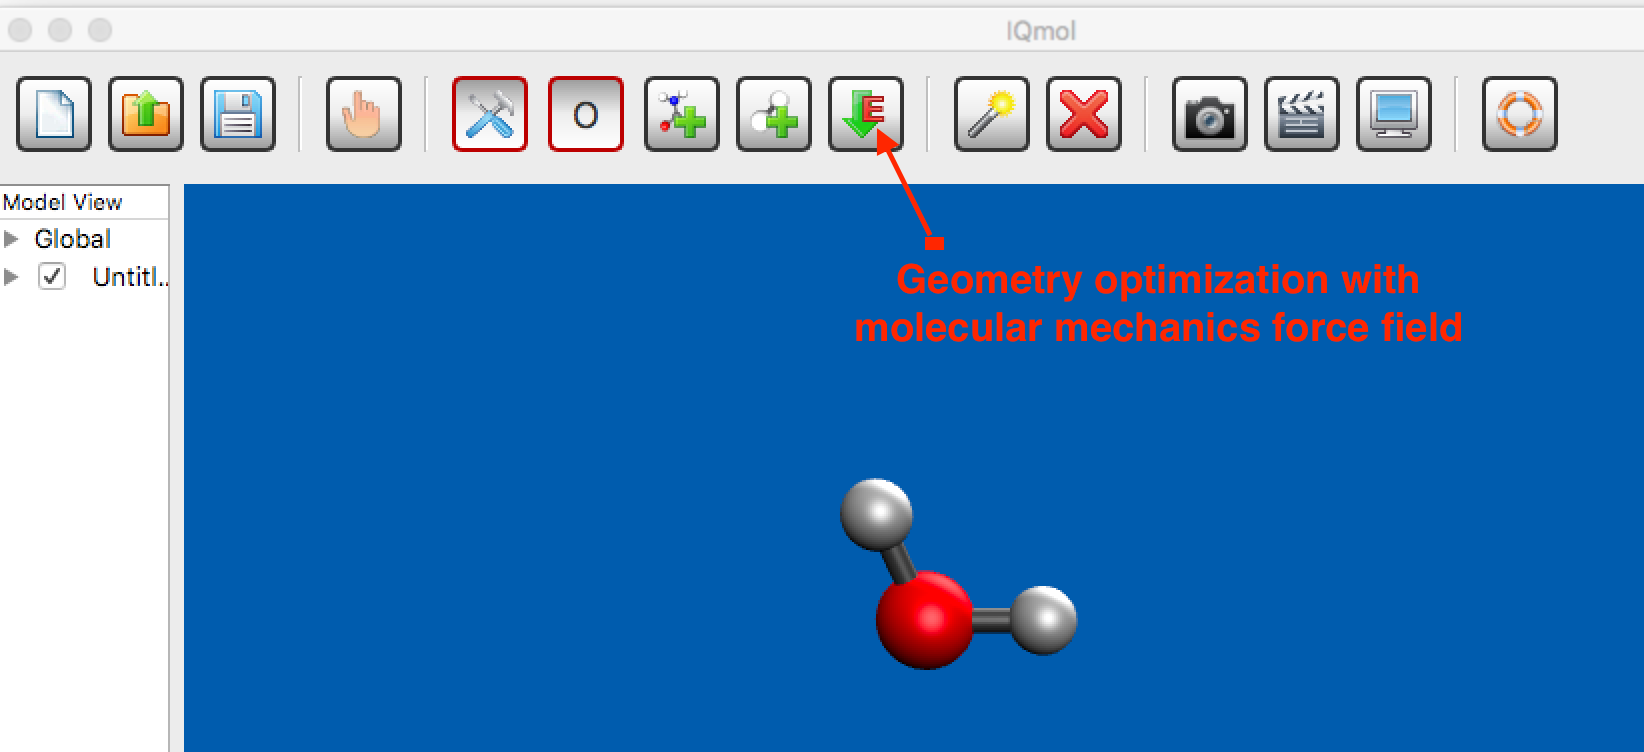
\includegraphics[height=2.0in]{figures/iqmol-water.png}
\end{center}
\end{frame}

\begin{frame}
\frametitle{Case Study: Water Molecule}
\begin{itemize}
\item Use IQmol to run Hartree-Fock/3-21G calculation
\end{itemize}
\begin{center}
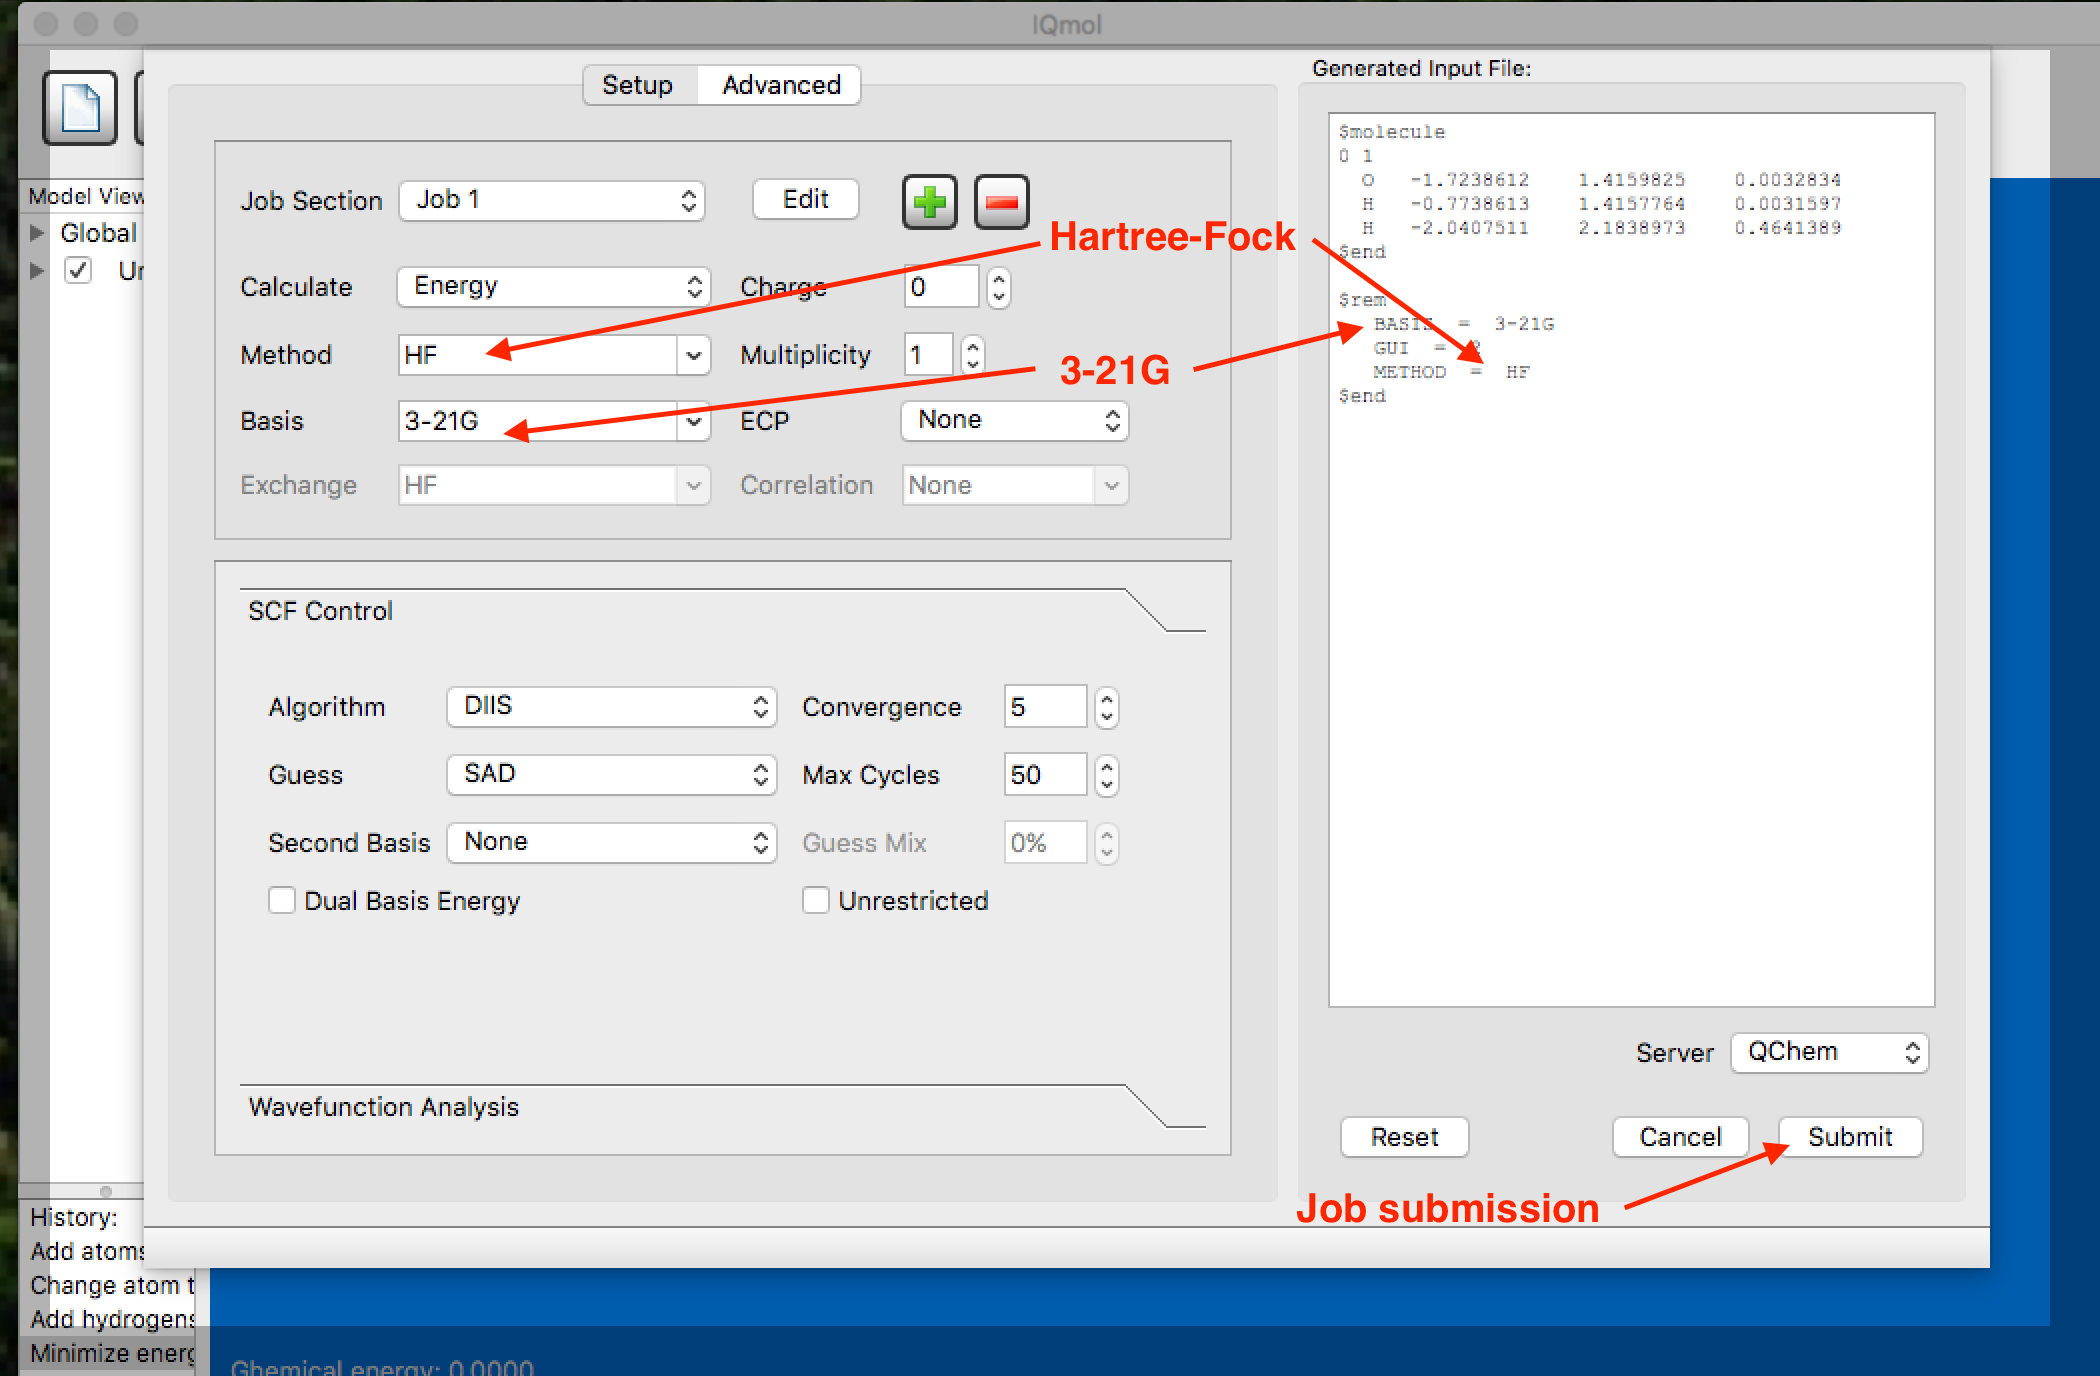
\includegraphics[height=2.5in]{figures/iqmol-water2.png}
\end{center}
\end{frame}

\begin{frame}
\frametitle{Case Study: Water Molecule}
\begin{itemize}
\item In IQmol, open the output file to draw a water molecule
\item Find Hartree-Fock total and orbital energies
\end{itemize}
\begin{center}
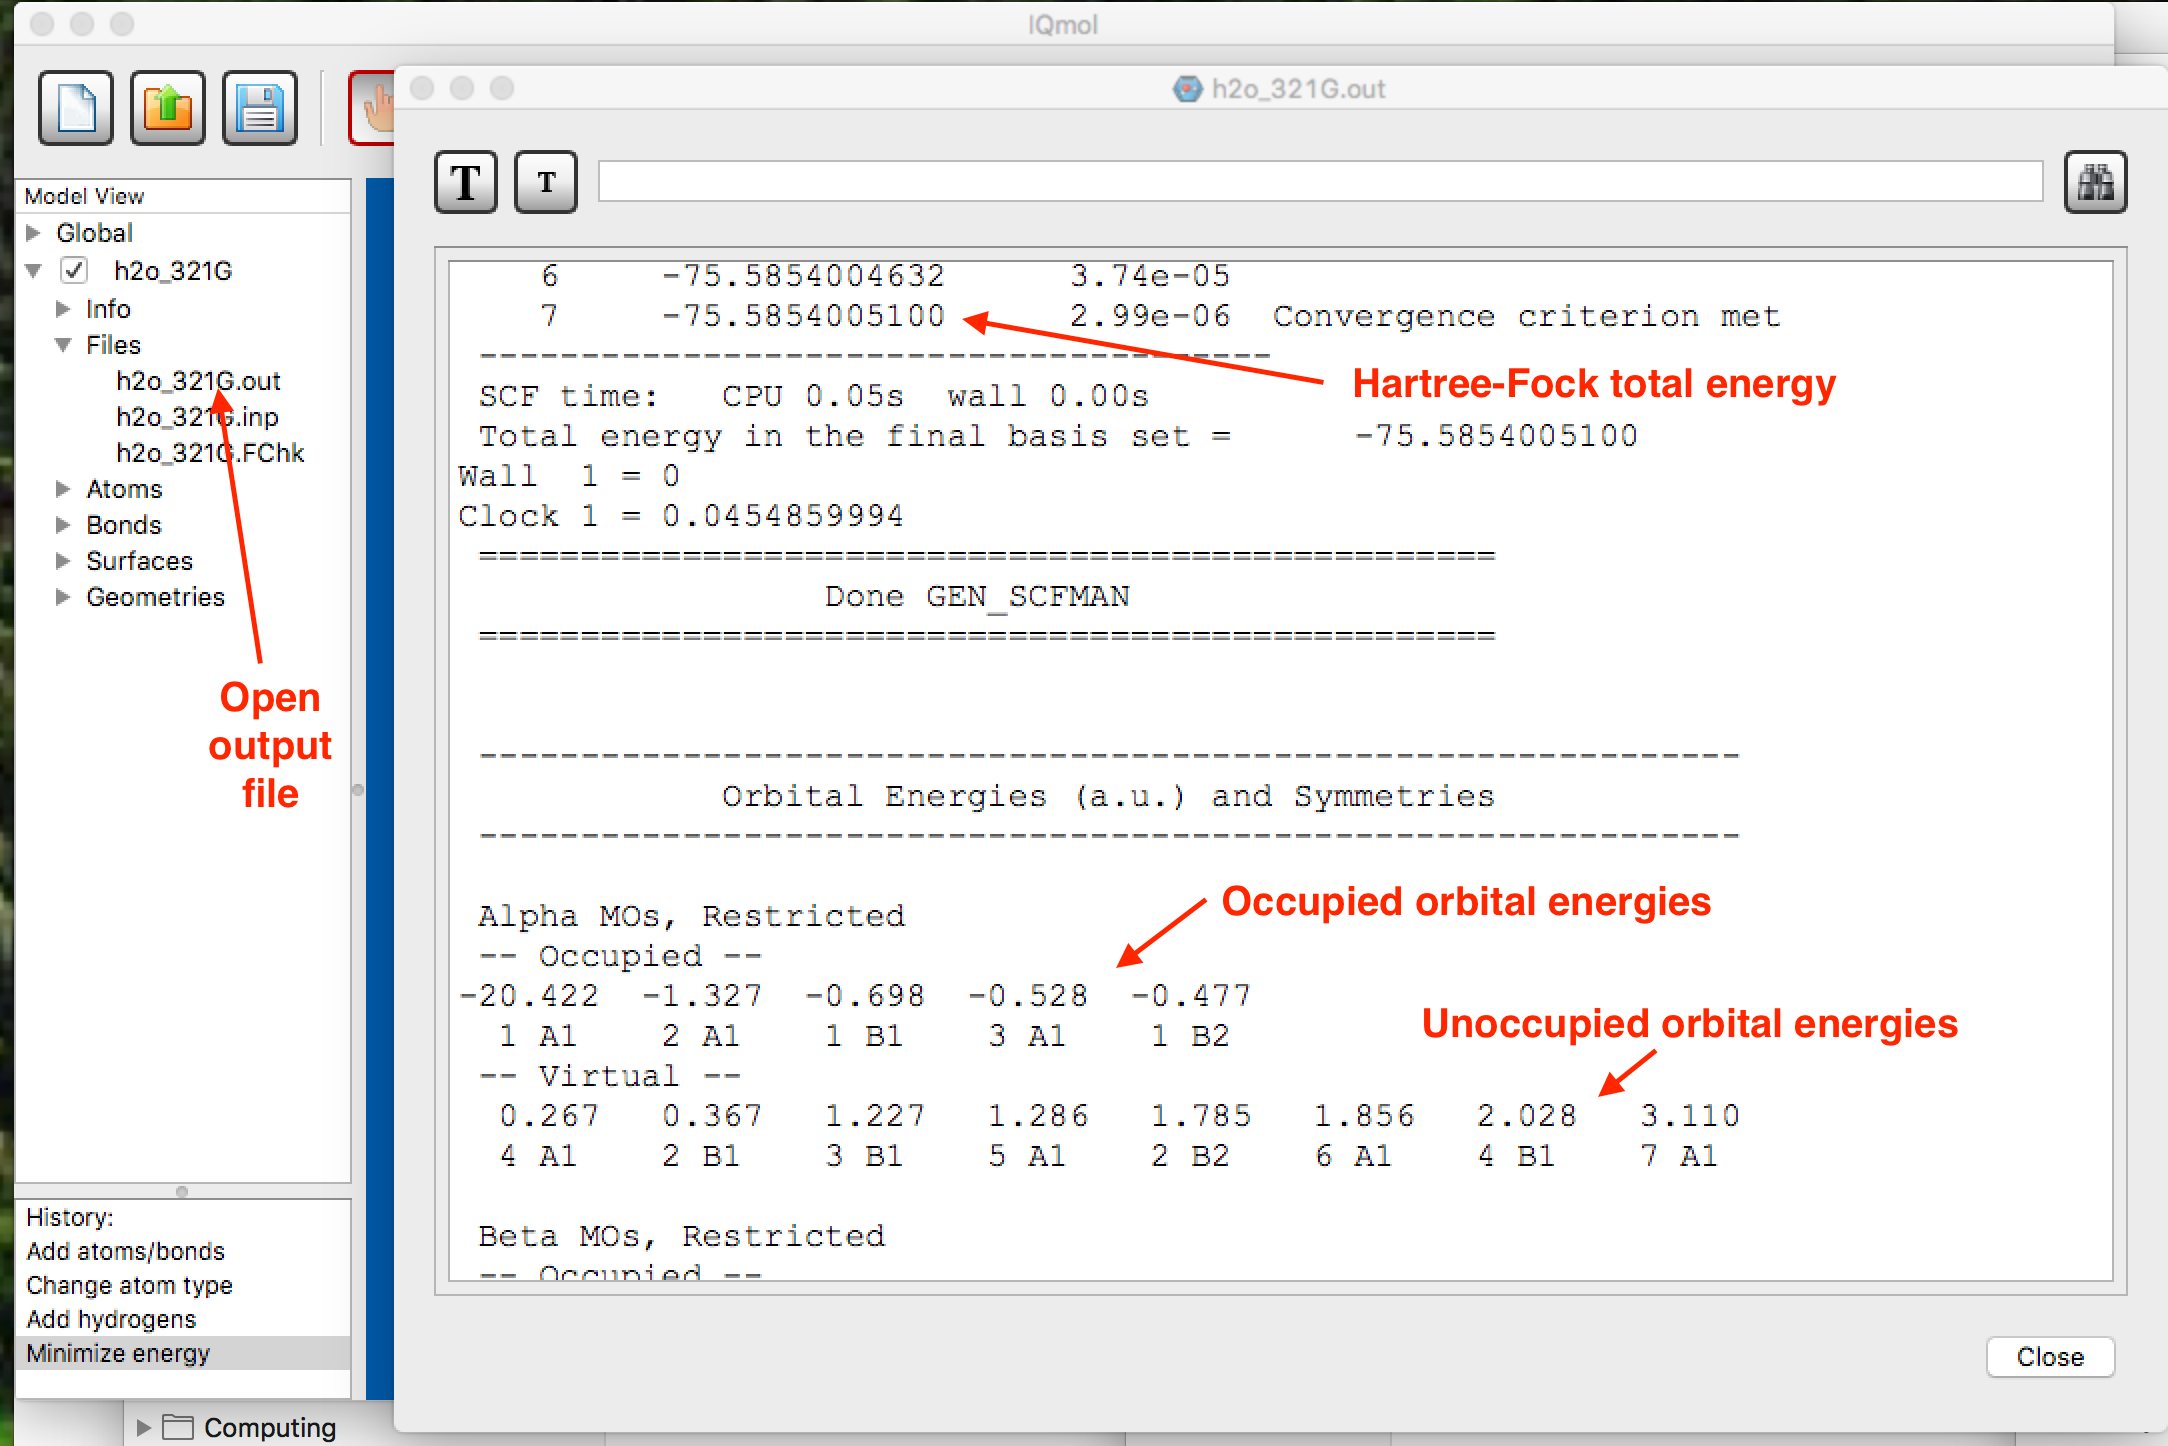
\includegraphics[height=2.0in]{figures/iqmol-water3.png}
\end{center}
\end{frame}

\begin{frame}
\begin{itemize}
\item Go to schooner, and make a new folder 
\item Copy 
\begin{itemize}
\item /home/yihan/qm\_tutorial/qchem\_files/FCIDump
\item /home/yihan/qm\_tutorial/python\_files/read\_fcidump.py
\end{itemize}
to the new folder.
\item Compute the Hatree-Fock total and orbital energies  
\end{itemize}
\end{frame}

\begin{frame}
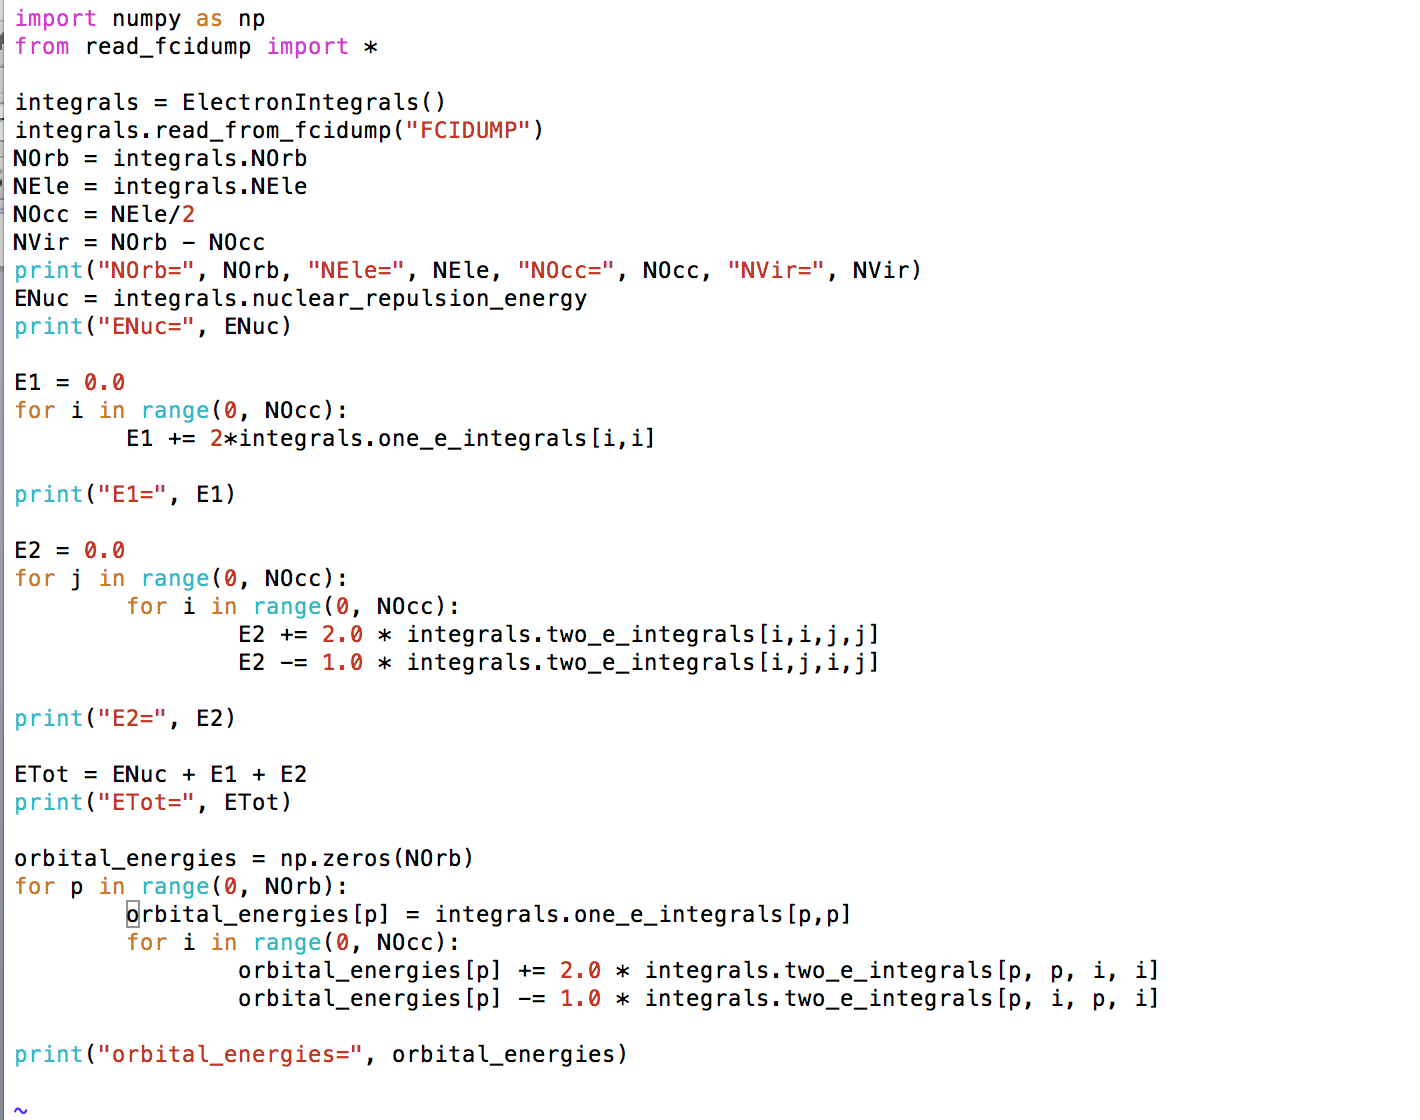
\includegraphics[height=3.0in]{figures/hf-energy-code.png}
\end{frame}

\end{document}

